\begin{multicols}{3}Гимназия "Гьоте"-синоним на стабилност, сигурност и просперитет"
\byline{Интервю с г-жа Ананиева, зам. кмет по култура и образование в община Бургас}{Пламена и Симеон, 10 Е}

\noindent 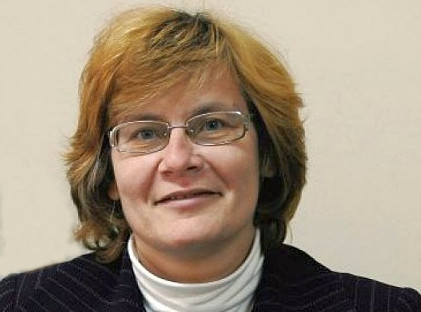
\includegraphics[width=2.1in]{./Ananieva/5.jpg}
Какво е Вашето мнение за ГПНЕ „Гьоте” в образователното пространство на 
общината? Виждате ли някаква разлика в образователния процес отпреди пет години 
и сега?
В мен името на гимназия „Гьоте“ предизвиква няколко асоциации: стабилност, 
сигурност и просперитет. Мисля, че в последните години освен, че са се сменили 
много колеги, се е развила възможността за работа в креативна посока и има много 
разчупени форми на дейност в различни посоки, финансирани не само от общината, 
но и от самата гимназия.
Смятате ли, че в днешно време нивото на българското образование се променя?
Аз смятам, че има нужда от  промени в нашата образователна система, защото 
днешното поколение ученици са много по-различни от поколението преди десет и 
повече години. Вие имате достъп до много повече източници на информация и имате 
възможност за повече комуникация, което дава един много по-широк кръгозор. 
Мисля, че нашата образователна система изостава от това, което е потребно за 
младите хора. Смятам, че много бързо трябва да се променят образователните 
планове, за да може придобитите знания да ви са от полза в сегашния свят.
Смятате ли, че има разлика в образователния процес?
Да, има, но смятам, че плановете в образователната система изостават. Реална 
промяна има при Вас, защото участвате в много проекти и извънкласни дейности.
Каква е стратегията на общината за подпомагане на училища като гимназия „Гьоте” 
и на изявените и талантливи ученици в него?
Община Бургас има много политики в областта на образованието. Една от нашите 
цели е свързана с подобряване на материалната база. Ние отговаряме за това, вие 
да имате добри условия за обучение-да имате отоплени сгради и хубави спортни 
площадки. Другото нещо, което е важно за нас е да подпомагаме изявите на 
различни ученици, включително и учениците от Немска гимназия. Всяка година 
община Бургас награждава учениците, които са достигнали високи резултати. 
Подпомагаме изявите на различни формации като вашия танцов състав, тетралната ви 
група. Има и други форми на партньорство с нас, но когато се научим да работим в 
екип, резултатите от общата ни дейност ще бъдат по-високи.
Предвижда ли се отделяне на Немска и Английска гимназии в отделни сгради, защото 
това са две големи училища с над 1600 ученици общо, а се помещават в една малка 
сграда, с капацитет за 400 ученици?  
Да, така е. Няколко са гимназиите, които се помещават в общи сгради. Вие сте 
училище с доказани във времето успехи, не е невъзможно отделянето на двете 
гимназии в самостоятелни сгради, но това не стои засега на дневен ред. Ако бъде 
приет новият закон за училищата, според който се разрешава прием от 5 клас  в 
езиковите гимназии, със сигурност ще се мисли  за нова сграда или преустрояване 
на вече съществуващата.
Обмисля ли се преустройство на физкултурния ни салон, защото ни се случва 4 
класа да имаме едновременно час в него и мястото е недостатъчно?
Има изготвен такъв финансов и инвестиционен план за разширение, но не стои на 
дневен ред осъществяването му. 
Поддържате ли по-тесни контакти с нашата гимназия?
Аз съм свързана емоционално с гимназията. Моята дъщеря завърши Немската 
гимназия. Поддържам контакти и с колегите от гимназията и си съдействаме 
взаимно.
Вашето пожелание по случай нашия юбилей?
За Вашия юбилей пожелавам, гимназията да продължи да създава в обществото и в 
нейните възпитаници чувството за сигурност, разкрепостеност и креативност. На 
всички завършващи тази гимназия пожелавам да реализират своите мечти и да имат 
нови, защото това движи човекът напред.
\closearticle
\end{multicols}
